% include research and teaching experience
\documentclass[12pt]{letter}
\usepackage[utf8]{inputenc}
\usepackage[bottommargin=1in]{CustomCoverletter}

\begin{document}

\begin{minipage}[c]{0.7\textwidth}
    \textbf{\LARGE \name~{\color{highlight}|} Curriculum Vitae}\vspace{0.5em}\\
    \role~at Lamarr-Institute | TU Dortmund University\\
    Born \birthinfo. Nationality: \nationality\\
    Email: \href{mailto:\mail}{\mail}\\
    To learn about my ongoing activities, visit my \href{\website}{webpage} and \href{\linkedin}{LinkedIn}\\
    My publications and software are listed on \href{\scholar}{Google Scholar} and \href{\github}{GitHub}\\
\end{minipage}\hfill%
\begin{minipage}[c]{0.29\textwidth}
    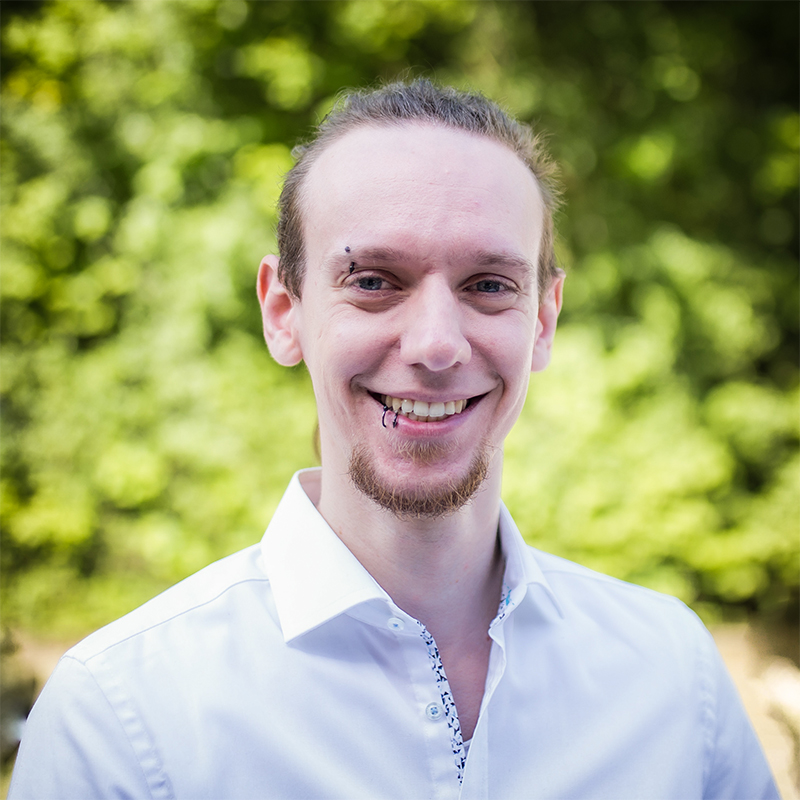
\includegraphics[width=.7\linewidth]{picture.jpg}
\end{minipage}

My research focuses on the \textbf{sustainability and trustworthiness of AI}, exploring implications for our society, economy, and environment.
Guided by interdisciplinarity and real-world applications, my \href{https://doi.org/10.17877/DE290R-25716}{PhD} contributed new methods for benchmarking, reporting, labeling, and meta-learning, accompanied by practical solutions from the \href{https://lamarr-institute.org/news/partnership-lamarr-institute-and-wilo/}{transfer project} with \emph{Wilo}.
I also lead the \href{https://youngaileaders-dortmund.de/}{\emph{Young AI Leaders Dortmund}}, under the UN \href{https://aiforgood.itu.int/young-ai-leaders-community/}{\emph{AI for Good}} mission.





\section{Professional Experience}

\begin{tabularx}{\textwidth}{p{0.14\textwidth}@{\hspace{1em}}X@{}}
  \textbf{06/19 -- Today} & \textbf{AI Scientist} @ Lamarr Institute for ML and AI (Dortmund)\\[-0.9em]
    & \footnotesize \begin{itemize}[leftmargin=1.2em,noitemsep,topsep=0pt]
        \item Researching on sustainability, resource-awareness and trustworthiness of AI
        \item 14 peer-reviewed publications, conference and delegation visits, transfer and network activities
      \end{itemize}
\end{tabularx}
\begin{tabularx}{\textwidth}{p{0.14\textwidth}@{\hspace{1em}}X@{}}
  \textbf{02/22 -- 03/25} &
    \textbf{Data Scientist (part time)} @ Wilo SE (Dortmund)\\[-0.9em]
    & \footnotesize \begin{itemize}[leftmargin=1.2em,noitemsep,topsep=0pt]
        \item Working in the strategic partnership with Lamarr Institute (research transfer project)
        \item Exploring AI use cases and prototyping ML solutions for industrial manufacturing
      \end{itemize}
\end{tabularx}
\begin{tabularx}{\textwidth}{p{0.14\textwidth}@{\hspace{1em}}X@{}}
  \textbf{07/16 -- 08/18} &
    \textbf{Working Student} @ Capgemini (Düsseldorf) \& Qiagen (Hilden)\\[-0.9em]
    & \footnotesize \begin{itemize}[leftmargin=1.2em,noitemsep,topsep=0pt]
        \item Software development for DNA sequencing, logging and testing with Qiagen as a client
      \end{itemize}
\end{tabularx}






\section{Education}

\begin{tabularx}{\textwidth}{p{0.14\textwidth}@{\hspace{1em}}X@{}}
  \textbf{06/19 -- 07/25} & \textbf{PhD in Computer Science} @ TU Dortmund University -- \emph{Summa cum laude} | 1.0 | ECTS A\\[-0.9em]
   & \footnotesize \begin{itemize}[leftmargin=1.2em,noitemsep,topsep=0pt]
        \item \textbf{Topic}: \emph{Advancing the Sustainability of ML and AI via Labeling and Meta-Learning}~\cite{fischer_advancing_2025}
        \item \textbf{Committee}: JProf. Thomas Liebig, Prof. Geoff Webb, Prof. Christian Janiesch, Prof. Jakob Rehof
      \end{itemize}
\end{tabularx}
\begin{tabularx}{\textwidth}{p{0.14\textwidth}@{\hspace{1em}}X@{}}
  \textbf{01/25 -- 03/25} & \textbf{Research Visit} @ Monash University, Melbourne\\[-0.9em]
   & \footnotesize \begin{itemize}[leftmargin=1.2em,noitemsep,topsep=0pt]
        \item Exploring resource efficiency in time series classification
      \end{itemize}
\end{tabularx}
\begin{tabularx}{\textwidth}{p{0.14\textwidth}@{\hspace{1em}}X@{}}
  \textbf{10/16 -- 03/19} & \textbf{Master's in Computer Science} @ TU Dortmund University -- \emph{Magna cum laude} | 1.2 | ECTS B\\[-0.9em]
    & \footnotesize \begin{itemize}[leftmargin=1.2em,noitemsep,topsep=0pt]
        \item \textbf{Topic}: \emph{Filling Gaps in Incomplete Satellite Images with Compressable STRFs}~\cite{fischer_filling_2019}
        \item \textbf{Supervisors}: Prof. Katharina Morik, Dr. Nico Piatkowski
      \end{itemize}
\end{tabularx}
\begin{tabularx}{\textwidth}{p{0.14\textwidth}@{\hspace{1em}}X@{}}
  \textbf{09/18 -- 03/19} & \textbf{Research Visit} @ Monash University, Melbourne\\[-0.9em]
   & \footnotesize \begin{itemize}[leftmargin=1.2em,noitemsep,topsep=0pt]
        \item Exploring probabilistic gap filling and cloud removal for satellite image series
      \end{itemize}
\end{tabularx}
\begin{tabularx}{\textwidth}{p{0.14\textwidth}@{\hspace{1em}}X@{}}
  \textbf{10/13 -- 09/16} &
    \textbf{Bachelor's in Computer Science} @ TU Dortmund University -- \emph{Cum laude} | 2.4 | ECTS C%\\[-0.9em]
    % & \small \begin{itemize}[leftmargin=1.2em,noitemsep,topsep=0pt]
      %   \item \textbf{Minor subject}: Spatial Planning
      % \end{itemize}\\[1em]
\end{tabularx}







\section{Awards \& Scholarships}

\begin{tabularx}{\textwidth}{p{0.07\textwidth}@{\hspace{1em}}X@{}}
  \textbf{2024} & \textbf{Sustainability Award of the Computer Science Faculty @ TU Dortmund University}\\[-0.9em]
   & \footnotesize \begin{itemize}[leftmargin=1.2em,noitemsep,topsep=0pt]
        \item awarded for our work on \emph{Sustainable LLMs: Energy Efficiency and Transparent Labeling}
      \end{itemize}\\
  \textbf{2014} & \textbf{Scholarship from the \emph{German Academic Scholarship Foundation (Studienstiftung)}}\\[-0.9em]
   & \footnotesize \begin{itemize}[leftmargin=1.2em,noitemsep,topsep=0pt]
        \item for my Bachelor's and Master's studies, also volunteering as \textbf{Regional Representative} (06/15 -- 06/17)
      \end{itemize}
\end{tabularx}







% \section{Core Research Topics}
% {\footnotesize
% \begin{tabularx}{\textwidth}{p{0.14\textwidth}@{\hspace{1em}}X@{}}
%   \textbf{2025 -- Today} & Investigating AI Potential for Political Education~\cite{fischer_benefits_2025}
% \end{tabularx}
% \begin{tabularx}{\textwidth}{p{0.14\textwidth}@{\hspace{1em}}X@{}}
%   \textbf{2023 -- Today} & Resource-Aware and User-Centric AutoML \& Meta-Learning~\cite{fischer_autoxpcr_2024,fischer_metaqure_2024}
% \end{tabularx}
% \begin{tabularx}{\textwidth}{p{0.14\textwidth}@{\hspace{1em}}X@{}}
%   \textbf{2022 -- Today} & Benchmarking Resource-Efficiency and Sustainability in AI~\cite{fischer_unified_2022,fischer_towards_2024,van_der_staay_stress-testing_2024,fischer_ground-truthing_2025}
% \end{tabularx}
% \begin{tabularx}{\textwidth}{p{0.14\textwidth}@{\hspace{1em}}X@{}}
%   \textbf{2021 -- Today} & AI Labels for Transparency and Trustworthiness~\cite{morik_care_2021,morik_yes_2022,fischer_bridging_2025,van_der_staay_reflective_2025}
% \end{tabularx}
% \begin{tabularx}{\textwidth}{p{0.14\textwidth}@{\hspace{1em}}X@{}}
%   \textbf{2022 -- 2025} & AI for Industrial Pump Manufacturing~\cite{fischer_prioritization_2023}
% \end{tabularx}
% \begin{tabularx}{\textwidth}{p{0.14\textwidth}@{\hspace{1em}}X@{}}
%   \textbf{2019 -- 2020} & Probabilistic Gap Filling in Satellite Imagery~\cite{fischer_parameter_2019,fischer_no_2020}
% \end{tabularx}}

\newpage




\section{Teaching Experience}

\textbf{Supervision} (Bachelor's \& Master's theses as well as student assistants)\\[-1.5em]
{\footnotesize \begin{itemize}[leftmargin=1.2em,noitemsep,topsep=0pt]
    \item[] 01/26 -- Master's student assistant Y. Abdelrahim, working on efficiency benchmarking of AI (ongoing)
    \item[] 10/25 -- BA of F. Meree on \emph{Interactive AI Labels for Trust: A User-Centric Reporting Framework}
    \item[] 06/24 -- Bachelor's student assistant K. Poitz, working on interdisciplinary evaluations of AI labels (ongoing)
    \item[] 10/24 -- BA of F. Theiner on \emph{Resource Efficiency of Adversarial Training and Inference of RobustBench Models}
    \item[] 02/24 -- BA of A. Borowski on \emph{Energy Efficiency Analysis of Knowledge Graph Embedding Models}
    \item[] 12/22 -- Master's student assistant A. van der Staay, working on benchmarking AI edge devices (until 12/23)
    \item[] 11/23 -- BA of T. Kubiak on \emph{A Comparative Analysis of Parameter-Efficient-Fine-Tuning Methods in LLMs}
    \item[] 09/22 -- MA of F. Dillkötter on \emph{Automated Generation of Evaluation Tasks for ML Models}
\end{itemize}}
    
\textbf{Individual Lectures} (for Bachelor's, Master's \& PhD students)\\[-1.5em]
{\footnotesize \begin{itemize}[leftmargin=1.2em,noitemsep,topsep=0pt]
  \item[] 10/25 -- \textbf{Sustainable Development in the Age of AI} as part of the \emph{Computer Science and Sustainability} lecture series
  \item[] 10/25 -- \textbf{Fundamentals of Trustworthy AI} as part of the \emph{Data, Knowledge, and Context in ML and AI} lecture series
  \item[] 05/25 -- \textbf{Sustainability and AI} as part of the \emph{Introduction to Data Science II} lecture series
\end{itemize}}

\textbf{Other Activities} (educating school students \& general public)\\[-1.5em]
{\footnotesize \begin{itemize}[leftmargin=1.2em,noitemsep,topsep=0pt]
  \item[] 2025 -- Teaching \href{https://www.linkedin.com/posts/german-international-school-of-silicon-valley_ai-ki-aiweek-activity-7419934687802064896-hY7S}{GISSV} students (remote) and organizing workshops for \href{https://www.diwodo.de/events/nachhaltigkeit-im-zeitalter-kunstlicher-intelligenz-7624b277-a97b-47b0-a4e0-58097e4eb080/}{Digital Week Dortmund} and \href{https://lamarr-institute.org/news/girls-day-2025/}{Girls' Day} @ Lamarr
  \item[] 2024 -- Training course for teachers on the topic of   \href{https://app.fobizz.com/fortbildungen/2236-ki-fokus-umwelt-und-nachhaltigkeit/}{AI, Environment and Sustainability} (fobizz / remote) 
  \item[] 2023 -- Organizing workshops for \href{https://lamarr-institute.org/news/ai4schools-workshop-des-lamarr-instituts/}{AI4Schools} and \href{https://lamarr-institute.org/news/diwodo-2023-regional-and-international-interest-in-lamarr-institute-ai-research/}{Digital Week Dortmund} @ Lamarr
  % \item[] 11/19 -- Co-organized a school lesson in politics
\end{itemize}}








\section{Volunteering \& Activities}

\textbf{Young AI Leaders} (since 2025) -- initiative coordinated by the United Nations' \emph{AI for Good} platform
{\footnotesize
\begin{itemize}[leftmargin=1.2em,noitemsep,topsep=0pt]
    \item \href{https://aiforgood.itu.int/young-ai-leaders-community/}{Global network} that empowers young enthusiasts to drive positive change with AI (over 100 Hubs with more than 650 members)
    \item Founded and actively leading the \href{https://youngaileaders-dortmund.de/}{Dortmund Hub}, growing to 15 members
    \item Investigating the use of \href{https://dortmund-wahl-ki.de/}{generative AI for political education} in context of the Dortmund municipal elections
\end{itemize}}

\textbf{Scientific Community Services} (since 2022) -- program-chairing and reviewing for
{\footnotesize
\begin{itemize}[leftmargin=1.2em,noitemsep,topsep=0pt]
    \item ACM Conference on Fairness, Accountability, and Transparency (FAccT) 2026
    \item Explainable AI for Time Series and Data Streams Workshop (TempXAI @ ECML-PKDD) 2025 \& 2024
    \item AAAI/ACM Conference on AI, Ethics, and Society (AIES) 2025
    \item ACM SIGKDD Conference on Knowledge Discovery and Data Mining (KDD) 2024
    \item European Conference on ML and Principles and Practice of Knowledge Discovery in Databases (ECML-PKDD) 2022
\end{itemize}}

\textbf{Lamarr Institute} (since 2019) -- research \& transfer activities (in addition to regular conference attendance)
{\footnotesize
\begin{itemize}[leftmargin=1.2em,noitemsep,topsep=0pt]
    \item \textbf{Invited talks} at the 
        \href{https://enfield-project.eu/second-energy-green-ai-workshop/}{ENFIELD Energy \& Green AI Workshop} (11/25), 
        \href{https://www.iwe.uni-bonn.de/en/events/sustainable-ai-conference-2025}{Sustainable AI Conference}, (09/25), 
        \href{https://www.business.ruhr/veranstaltungen/greentechruhr-jahrestreffen.html}{Greentech.Ruhr meeting} (05/25), 
        \href{https://www.linkedin.com/posts/lamarr-institut_dopplers2025-physics-artificialintelligence-activity-7313145002610589698-WCun}{DOPPLERS} (03/25),
        \href{https://lamarr-institute.org/events/ki-werkstatt-2024/}{BAuA KI-Werkstatt} (11/24),
        \href{https://2023-aisola.isola-conference.org/}{AISoLA Conference} (10/23),
        and \href{https://lamarr-institute.org/news/all-hands-meeting-of-the-german-ai-centers/}{BIFOLD All Hands Meeting} (10/23)    
    \item \textbf{Posters \& demos} at the \href{https://www.trustworthy-ai-summit.eu/}{Trustworthy AI Summit} (09/25), 
        \href{https://lamarr-institute.org/news/bmbf-state-secretary-mario-brandenburg-and-mkw-state-secretary-gonca-turkeli-dehnert-visit-lamarr-institute/}{political visits} (06/24), (09/23), (08/19), and various \href{https://www.linkedin.com/posts/lamarr-institut_serbia-exchange-europeanai-activity-7405182012350758913-zr-F}{strategic events} % (11/25), (05/24), (06/21), (01/20)
    \item \textbf{Selected delegation member} for visiting institutions in \href{https://lamarr-institute.org/news/canada-delegation-pressrelease/}{Canada} (10/25), \href{https://lamarr-institute.org/news/usa-delegation-trip/}{USA} (04/24), and \href{https://www.ml2r.de/en/franco-german-workshop-on-artificial-intelligence/}{France} (07/22)
    \item \textbf{Research visit \& talk} at Emma Strubell's Lab @ Carnegie Mellon University, Pittsburg, USA (02/22)
    \item Contributed four \href{https://lamarr-institute.org/de/person/fischer-raphael/}{posts to the ML Blog}~\cite{fischer_optimization_2021,fischer_preparation_2021,fischer_energy_2023b,poitz_ai_2025}
    \item Active participation in various \textbf{Lab Visits}, \textbf{Scientific Forums}, \textbf{Pitch Talks}, and \textbf{Education Activities} (2020 -- 2026)
\end{itemize}}

\textbf{CS Faculty @ TU Dortmund University} -- engaging in administrative activities
{\footnotesize
\begin{itemize}[leftmargin=1.2em,noitemsep,topsep=0pt]
    \item \textbf{Sustainability Commission}: Conducting and promoting sustainable efforts (06/2025 -- Today)
    \item \textbf{International Coordination}: Assisting students and employees with stays abroad (12/2020 -- 12/2025)
    \item \textbf{Faculty Council}: Representative of the research associates (2022 -- 2024)
\end{itemize}}

\newpage

\nocite{*}
\renewcommand*{\bibfont}{\small}
\printbibliography[title={Peer-Reviewed Publications},category=peerreviewed]
\printbibliography[title={Preprints and Gray Literature},category=preprint]
\printbibliography[title={Videos \& Recorded Talks},category=videotalks]

\end{document}